\lab{The Finite Element method}{The Finite Element method}
\label{lab:finite_element}
\objective{The finite element method is commonly used for numerically solving partial differential equations. We introduce the finite element method via a simple BVP describing the steady state distribution of heat in a pipe as fluid flows through.}
\labdependencies{FiniteDifferenceMethod}

\section*{Advection-Diffusion of Heat in a Fluid}

%%%% Old explanation
\begin{comment}
We begin with the heat equation
\begin{align*}
y_t = \epsilon y_{xx} + f(x) %\label{FEM:diffusion}
\end{align*}
where $f(x)$ represents any heat sources in the system, and $\epsilon y_{xx}$ models the diffusion of heat.
We wish to study the distribution of heat in a fluid that is moving at some constant speed $a$.
This can be modelled by adding an \textit{advection} or \textit{transport} term to the heat equation, giving us
\begin{align*}
y_t + ay_x = \epsilon y_{xx} + f(x).
\end{align*}
We consider the scenario of a fluid flowing through a pipe from $x = 0$ to $x = 1$ with  speed $a = 1$, and as it travels it is warmed at a constant rate $f= 1$.
Suppose that the fluid is already at a known temperature \(y=2\) as it enters the pipe.
This imposes the boundary condition \(y(0)=2\).

These conditions yield 
\begin{align*}
	&{ } y_t + y_x = \epsilon y_{xx} + 1, \quad 0 < x < 1, \\
	&{ } y(0) = 2
\end{align*}
As time progresses, we expect the temperature of the fluid in the pipe to reach a steady state distribution, with $y_t = 0$. The heat distribution then satisfies 
\begin{align*}
\begin{split}
&{ } \epsilon y'' - y' = -1, \quad 0 < x < 1,\\
&{ } y(0) = 2.
\end{split}
\end{align*}
This problem is not fully specified, since it is a linear second-order ODE but has only one boundary condition.
Suppose a device is installed on the end of the pipe that nearly instantaneously brings the heat of the water up to $y = 4$.
Physically, we expect this extra heat that is introduced at $x = 1$ to diffuse backward through the water in the pipe. This leads to a well defined BVP 
\begin{align}
	\begin{split}
	&{ } \epsilon y'' - y' = -1, \quad 0 < x < 1, \\
	&{ } y(0) = 2, \quad y(1) = 4.
	\end{split}\label{eqn:FEM_steady_state}
\end{align}
\end{comment}

%%%%%%%%%%

We wish to study the distribution of heat in a fluid that is moving at some constant speed $a$.
Let \(y\) denote the temperature of the fluid at any given location and time.
The equation modeling this situation can be obtained from the differential form of the conservation law, where the flux is the sum of a diffusive term \(-\epsilon y_x\) and an advection (or transport) term \(ay\):
\[
J = ay - \epsilon y_x
\]
The one-dimension conservation law states that \(y\) must then obey the partial differential equation \(
y_t + J_x = f(x)
\), where \(f\) represents heat sources in the system.
Since \(J_x = ay_x-\epsilon y_{xx}\), we obtain the \textit{advection-diffusion equation}
\begin{align*}
y_t+ay_x &=\epsilon y_{xx} +  f(x).
\end{align*}
As time progresses, we expect the temperature of the fluid in the pipe to reach a steady state distribution, with $y_t = 0$.
Once this steady state has been reached, the heat distribution \(y\) then satisfies the ODE
\begin{align*}
\epsilon y'' -ay' = -f(x).
\end{align*}

We consider the scenario of a fluid flowing through a pipe from $x = 0$ to $x = 1$ with  speed $a = 1$, and as it travels it is warmed at a constant rate $f(x)= 1$.
Note that since this a second-order ODE, we need two boundary conditions.
Suppose that the fluid is already at a known temperature \(y=2\) as it enters the pipe.
This imposes the boundary condition \(y(0)=2\).
Suppose further that a device is installed on the end of the pipe that nearly instantaneously brings the heat of the water up to $y = 4$.
Physically, we expect this extra heat that is introduced at $x = 1$ to diffuse backward through the water in the pipe and thus influence the steady-state temperature.
Putting this together leads to a well defined BVP:
\begin{align}
	\begin{split}
	&{ } \epsilon y'' - y' = -1, \quad 0 < x < 1, \\
	&{ } y(0) = 2, \quad y(1) = 4.
	\end{split}\label{eqn:FEM_steady_state}
\end{align}
The analytic solution for \(\epsilon=0.1\) is shown in Figure \ref{fig:FEM_analytic_solution}.

\begin{figure}[ht]
\centering
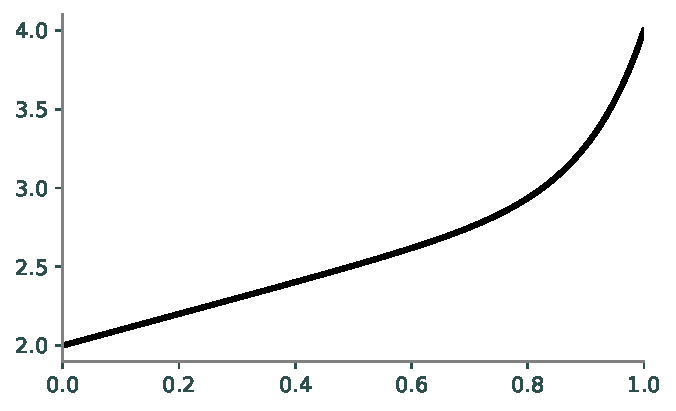
\includegraphics[width=\textwidth]{figures/FEM_solution.pdf}
\caption{The analytic solution of \eqref{eqn:FEM_steady_state} for $\epsilon = 0.1$.}
\label{fig:FEM_analytic_solution}
\end{figure}

\section*{The Weak Formulation}
Stepping back momentarily, consider the equation
\begin{align}
	\begin{split}
	&{ }\epsilon y'' - y' = -f, \quad 0 < x < 1,\\
	&{ }y(0) = \alpha, \quad y(1) = \beta .
	\end{split}\label{eqn:FEM_eqn1}
\end{align}
To approximate the solution $y$ using the finite element method, we reframe the problem into one involving integrals, known as its \textit{weak formulation}.

Let $w$ be a smooth function on $[0,1]$ satisfying $w(0) = w(1) = 0$.
Multiplying \eqref{eqn:FEM_eqn1} by $w$ and integrating over $[0,1]$ yields
\begin{align*}
	\int_0^1 -f w\,dx &= \int_0^1 (\epsilon y''w - y'w)\, dx, \\
	&= \int_0^1 (-\epsilon y'w' - y'w)\,dx,
\end{align*}
where the second equality follows by integration by parts.
For notational convenience, define the functionals $a$ and $l$ by
\begin{align*}
a(y,w) &= \int_0^1 -\epsilon y'w' - y'w\,dx,\\
l(w) &= \int_0^1 -f w\,dx.
\end{align*}
Then, any solution to \eqref{eqn:FEM_eqn1} will also satisfy
\begin{align}
	a(y,w) &= l(w)
	\label{eqn:FEM_integral_form}
\end{align}
This equation is the \textit{weak formulation} of \eqref{eqn:FEM_eqn1}.
Note that any solution to the original ODE is also a solution to the weak formulation.
However, solutions to the weak formulation need not be solutions to the original ODE, as they may not even be differentiable everywhere.
While this may seem like an undesirable property, it allows us to use a wider variety of functions to approximate the true solution.

Now, we choose some appropriate vector space \(V\) of functions, and consider the problem of finding a function $y\in V$ that satisfies the weak formulation \eqref{eqn:FEM_integral_form} for all $w\in V_0 = \{w \in V|w(0) = w(1) = 0\}$.
The \textit{finite element method} consists of choosing \(V\) to be some set of piecewise polynomial functions.
In this lab, we will consider the case of using piecewise linear functions.

\section*{The Finite Element Method}

Let $\mathrm{P}_n$ be some partition of $[0,1]$, $0 = x_0 < x_1< \ldots < x_{n} = 1$, and let $V_n$ be the set of continuous linear piecewise functions $v$ on $[0,1]$ such that $v$ is linear on each subinterval $[x_j,x_{j+1}]$.
These subintervals are the finite elements for which this method is named.
Note that $V_n$ has dimension $n+1$, since each of the continuous piecewise linear functions in $V$ are uniquely determined by their values at the \(n+1\) points \(x_0,x_1\ldots,x_n\).
Let $V_{n,0}$ be the subspace of $V_n$ of dimension $n-1$ whose elements are zero at the endpoints of $[0,1]$.
%We now seek to find a convenient basis for \(V_n\) in order to apply \eqref{eqn:FEM_integral_form}

%Now, consider $\{\mathrm{P}_n\}$ be a sequence of partitions that are refinements of each other, such that $\triangle x_n \to 0$ as $n \to \infty$.
%Then in particular $V_1 \subset V_2 \subset \ldots \subset V_n \ldots \subset V$.
%For each partition $\mathrm{P}_n$ we can find an approximation $y_n \in V_n$ for the true solution $y$; if this is done correctly then $y_n \to y$ as $n \to \infty$.

Let the $\phi_i$ be the hat functions 
\[\phi_i(x) = \begin{cases}
(x - x_{i-1})/h_i &\text{ if } x \in [x_{i-1},x_i]\\
 (x_{i+1} - x)/h_{i+1}  &\text{ if } x \in [x_{i},x_{i+1}]\\
0 &\text{ otherwise}
\end{cases}\]
where $h_i = x_i - x_{i-1}$; see Figures \ref{fig:FEM_one_basis_function} and \ref{fig:FEM_basis_functions}. 
These hat functions form a basis for $V_n$.
Note that the points \(x_0,\ldots,x_n\) need not be evenly spaced, and the \(h_i\) do not need to be equal.
This is in fact one of the major strengths of this approach, as it allows adapting the points in the partition to the problem, which can reduce the error in the approximation.
When applied to PDEs, it also is a simple way to handle unusually-shaped domains.

We now can write our approximate solution for \(y\) and the arbitrary function \(w\) as a linear combination of these basis elements, which will enable us to solve the system numerically.
In particular, we can write \(\hat{y}(x)=\sum_{i=0}^n k_i \phi_i(x)\), where the \(k_i\) are to be determined.

\begin{figure}[ht]
\centering
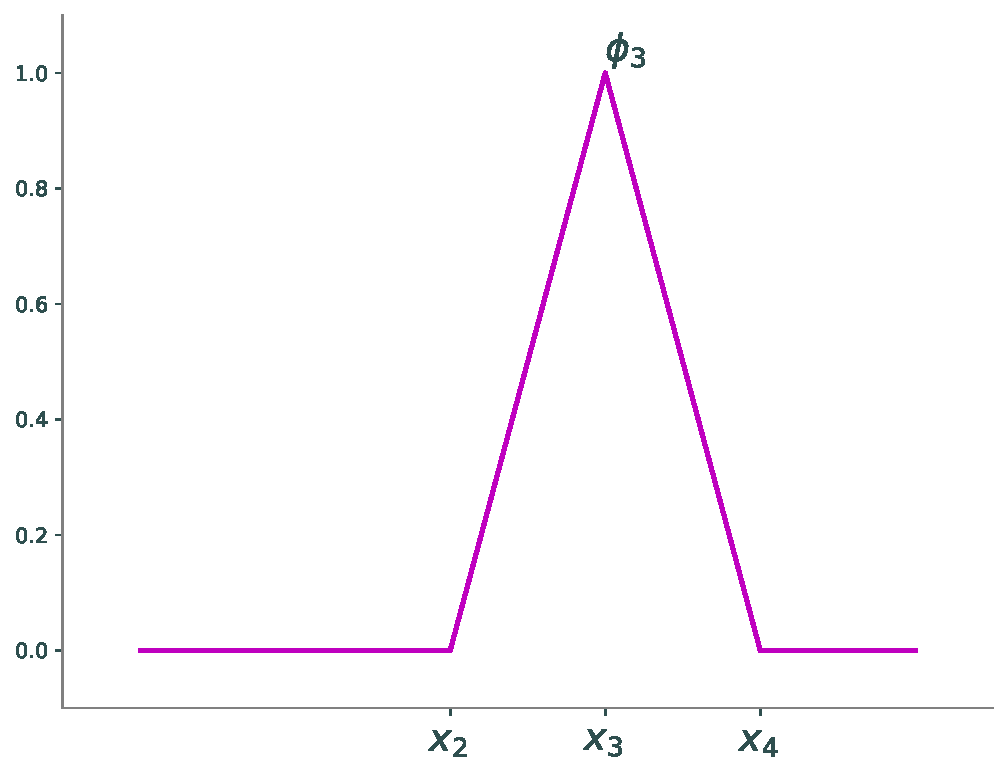
\includegraphics[width=\textwidth]{figures/one_basis_function.pdf}
\caption{The basis function $\phi_3$, when the \(x_i\) are evenly spaced.}
\label{fig:FEM_one_basis_function}
\end{figure}

\begin{figure}[ht]
\centering
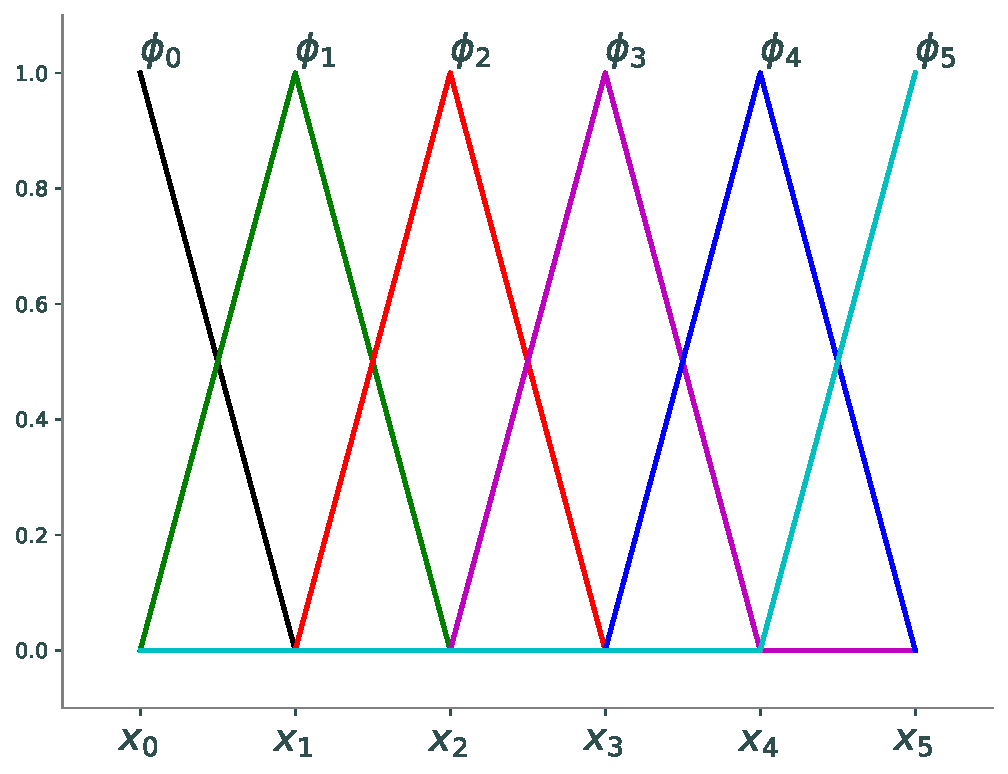
\includegraphics[width=\textwidth]{figures/basis_functions.pdf}
\caption{The six basis functions for $V_5$, when the \(x_i\) are evenly spaced.}
\label{fig:FEM_basis_functions}
\end{figure}

To make things more concrete, consider the case of \(n=5\) with the partition $\mathrm{P}_5 = \{x_0, x_1, \ldots, x_5\}$.
We look for an approximation $\hat{y} = \sum_{i=0}^5 k_i \phi_i \in V_5$ of the true solution $y$; to do this, we must determine appropriate values for the constants $k_i$.
We impose the condition on $\hat{y}$ that 
\[a(\hat{y},w) = l(w)\]
for all \(w \in V_{5,0}\).
This can be written equivalently as 
\[a \left( \sum_{i=0}^5 k_i \phi_i,\phi_j \right) = l(\phi_j) \quad \text{for } j = 1,2,3,4,\]
since \(a\) and \(l\) are linear in \(w\) and $\phi_1, \phi_2, \phi_3, \phi_4$ form a basis for $V_{5,0}$.
Since $a$ is also linear in \(y\), we further obtain 
\[\sum_{i=0}^5 k_i  a ( \phi_i,\phi_j ) = l(\phi_j) \quad \text{for } j = 1,2,3,4.\]
To satisfy the boundary conditions, we necessarily have that $k_0 = \alpha$, $k_5 = \beta$.
These equations can be written together in matrix form as
\begin{align} AK = \Phi,\label{eqn:FEM_linear_system}\end{align}
where
\begin{align}
A = \left[\begin{array}{cccccc}1 & 0 & 0 & 0 & 0 & 0 \\a(\phi_0,\phi_1) & a(\phi_1,\phi_1) & a(\phi_2,\phi_1) & 0 & 0 & 0 \\0 & a(\phi_1,\phi_2) & a(\phi_2,\phi_2) & a(\phi_3,\phi_2) & 0 & 0 \\0 & 0 & a(\phi_2,\phi_3) & a(\phi_3,\phi_3) & a(\phi_4,\phi_3) & 0 \\0 & 0 & 0 & a(\phi_3,\phi_4) & a(\phi_4,\phi_4) & a(\phi_5,\phi_4) \\0 & 0 & 0 & 0 & 0 &1\end{array}\right]
\label{eqn:FEM:A_matrix}
\end{align}
and
\begin{align}
K = \left[\begin{array}{c}k_0 \\k_1 \\k_2 \\k_3 \\k_4 \\k_5\end{array}\right] , \quad\Phi =  \left[\begin{array}{c}\alpha \\l(\phi_1) \\l(\phi_2) \\l(\phi_3) \\l(\phi_4) \\\beta\end{array}\right].
\label{eqn:FEM:K_Phi_definition}
\end{align}

Note that since $a(\phi_i,\phi_j) = 0$ for most values of $i, j$ (in particular, when the hat functions do not have overlapping domains), the finite element method results in a sparse linear system.
To compute the coefficients of \eqref{eqn:FEM_linear_system} we begin by evaluating some integrals.
Since
\begin{align*}
\phi_i(x) &= \begin{cases}
(x - x_{i-1})/h_i &\text{ if } x \in [x_{i-1},x_i]\\
 (x_{i+1} - x)/h_{i+1}  &\text{ if } x \in [x_{i},x_{i+1}]\\
0 &\text{ otherwise}
\end{cases}
\\
\phi_i'(x) &= \begin{cases}
1/h_i \quad \quad \quad \, \text{for } x_{i-1} < x < x_i,\\
 -1/h_{i+1} \quad \text{ for } x_{i} < x < x_{i+1},\\
0 \quad \quad \quad \quad \, \text{ otherwise},
\end{cases}
\end{align*}
we obtain
\begin{align*}
\int_0^1  \phi_i'\phi_j' &= \begin{cases}
- 1/h_{i+1} \quad \quad \quad \text{ if } j=i+1,\\
1/h_i + 1/h_{i+1} \quad \text{if } j=i,\\
0 \quad \quad \quad \quad \quad \quad \, \text{ otherwise},
\end{cases} \\
\int_0^1  \phi_i'\phi_j &= \begin{cases}
- 1/2 \quad \,\text{ if } j=i+1,\\
1/2 \quad \quad \text{ if } j=i-1,\\
0 \quad \quad \quad \text{ otherwise},
\end{cases}
\end{align*}
which can be put together to obtain (for \(f(x)=1\))
\begin{align}
a(\phi_i,\phi_j) &= \begin{cases}
\epsilon/h_{i+1} + 1/2 \quad \quad \, \text{ if } j=i+1,\\
-\epsilon/h_i -\epsilon/h_{i+1} \quad  \text{ if } j=i,\\
\epsilon/h_i - 1/2 \quad \quad \quad \, \text{ if } j=i-1,\\
0 \quad \quad \quad \quad \quad \quad \,\,\,\,\,\,\, \text{ otherwise},
\end{cases}
\label{eqn:FEM:a_definition}
\\
l(\phi_j) &= -\frac{1}{2}(h_j + h_{j+1}).
\label{eqn:FEM:l_definition}
\end{align}
Equation \eqref{eqn:FEM_linear_system} may now be solved using any standard linear solver. 
To handle the large number of elements required for Problem \ref{prob:FEM_accuracy_comparison}, you will want to use sparse matrices from \li{scipy.sparse}.

If you have become completely lost in the math at this point, do not fear.
To summarize, we need to solve \ref{eqn:FEM_linear_system} for $K$, where $A$ is defined by \ref{eqn:FEM:A_matrix} and $\Phi$ is defined in \ref{eqn:FEM:K_Phi_definition}.
The elements of $A$ and $\Phi$ are defined in \ref{eqn:FEM:a_definition} and \ref{eqn:FEM:l_definition}.
The vector $K$ is the approximated solution to the ODE given in \ref{eqn:FEM_exercise} and can be plotted very simply using \li{plt.plot(x, k)}, where \li{x} and \li{k} are arrays of the \(x_i\) and \(k_i\).
Note that $h_i$ is indexed from 1 to $N+1$, and that $h_i=x_i-x_{i-1}$.
You should now have everything you need to know to tackle the problems below.


\begin{problem}
Use the finite element method to solve
\begin{align}
	\begin{split}
	&{ }\epsilon y'' - y' = -1,\\
	&{ }y(0) = \alpha, \quad y(1) = \beta,
	\end{split} \label{eqn:FEM_exercise}
\end{align}
where $\alpha = 2, \beta = 4$, and $\epsilon = 0.02$.
Use $N = 100$ finite elements ($101$ grid points).
Compare your solution with the analytic solution
\[y(x) = \alpha + x + (\beta - \alpha - 1 ) \frac{e^{x/\epsilon} -1}{e^{1/\epsilon} -1}.\]

Hint: Make sure that your code does not assume that the grid points are evenly spaced.
\end{problem}

\begin{problem}
One of the strengths of the finite element method is the ability to generate grids that better suit the problem.
The solution of \eqref{eqn:FEM_exercise} changes most rapidly near $x = 1$.
Compare the numerical solution when the grid points are unevenly spaced versus when the grid points are clustered in the area of greatest change; see Figure \ref{fig:FEM_compare_methods}. Specifically, use the grid points defined by
\begin{lstlisting}
even_grid = np.linspace(0,1,15)
clustered_grid = np.linspace(0,1,15)**(1./8)
\end{lstlisting}
\end{problem}

\begin{figure}[ht]
\centering
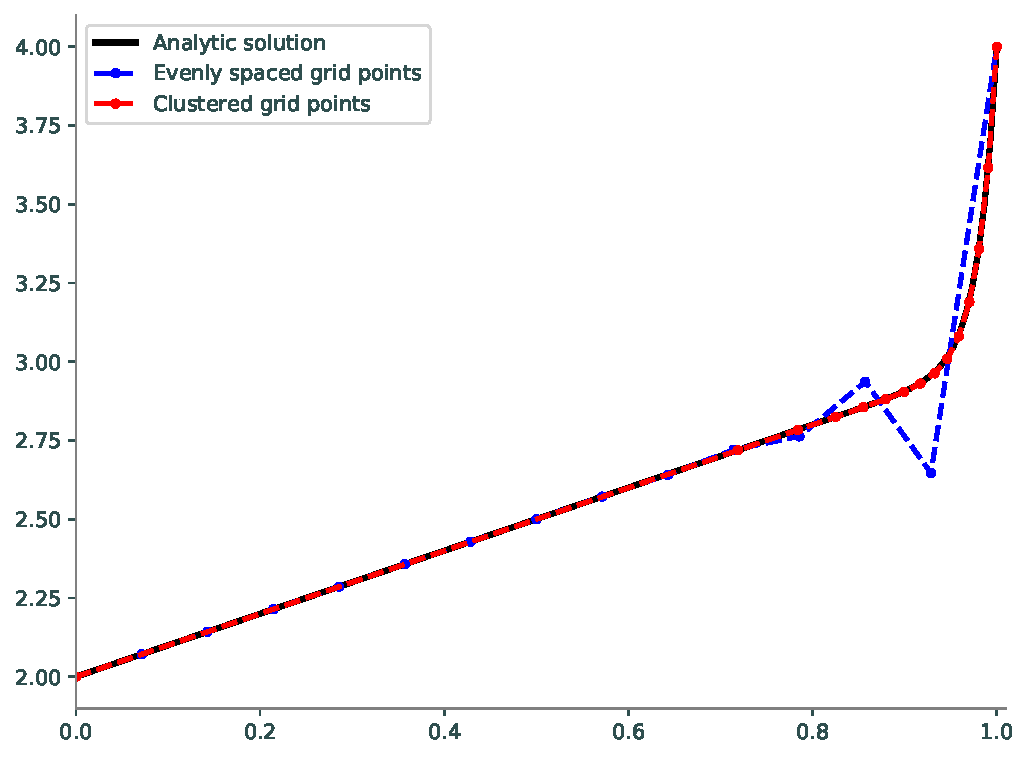
\includegraphics[width=\textwidth]{figures/FEM_compare_methods.pdf}
\caption{Two finite element approximations using 15 grid points, with different spacings. }
\label{fig:FEM_compare_methods}
\end{figure}

\begin{problem}
\label{prob:FEM_accuracy_comparison}
Higher order methods promise faster convergence, but typically require more work to code.
So why do we use them when a low order method will converge just as well, albeit with more grid points?
The answer concerns the roundoff error associated with floating point arithmetic.
Low order methods generally require more floating point operations, so roundoff error has a much greater effect.

The finite element method introduced here is a second order method, even though the approximate solution is piecewise linear.
(To see this, note that if the grid points are evenly spaced, the matrix $A$ in \eqref{eqn:FEM_linear_system} is exactly the same as the matrix for the second order centered finite difference method.)

Solve \eqref{eqn:FEM_exercise} with the finite element method using $N = 2^i$ evenly-spaced finite elements, $i = 4, 5, \ldots, 21$.
Remember to use sparse matrices, as this greatly reduces the memory and computation needed for the larger \(N\).
Compute the error as the maximum absolute value of the difference of the values of the approximate and true solutions at each of the \(x_i\).
Use a log-log plot to graph the error, and compare with Figure \ref{fig:FEM_error_2nd_order}.
\end{problem}


\begin{figure}[ht]
\centering
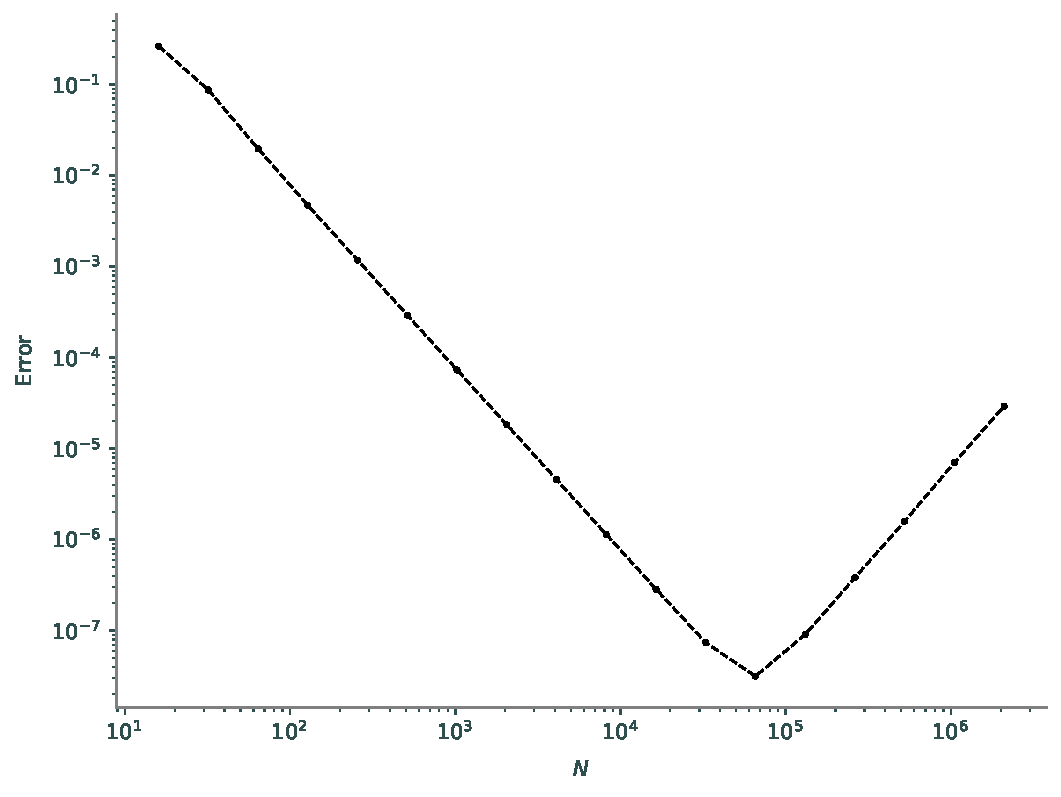
\includegraphics[width=\textwidth]{figures/FEM_error_2nd_order.pdf}
\caption{Error for the second order finite element method, as the number of subintervals $N$ grows. Round-off error eventually overwhelms the approximation. }
\label{fig:FEM_error_2nd_order}
\end{figure}

%\newpage
%\section*{A Comparison of Numerical Methods}
%
%\begin{table}[t]
%  \begin{tabular}{ l |l l }
%    % \hline
%     & Finite Element & Finite Difference  \\ \hline
%    Linear System& sparse& sparse  \\
%   Derivative & approximated locally & approximated locally \\
%Domain & irregular domains & fairly regular\\
%% Problem Formulation & integral & derivative & derivative & integral \\
%Convergence & polynomial & polynomial \\
%Strengths & adaptive mesh & easier to understand \\
%& refinement & and implement \\
%& complex geometries & easier for higher dimensions \\
%    \hline
%  \end{tabular}
%\end{table}
%
%\begin{table}
%  \begin{tabular}{ l |l l }
%    % \hline
%      & Pseudospectral & Finite Volume \\ \hline
%    Linear System & dense & sparse \\
%   Derivative & global & local\\
%Domain  & very nice & fairly regular\\
%Convergence  & exponential & polynomial\\
%Strengths  & fast convergence & handling discontinuities in \\
%& accurate to high precisions &the initial conditions \\
%& & dealing with shock formation \\
%& & and propagation \\
%    \hline
%  \end{tabular}
%\end{table}
%
%It is important to note that these methods are often mixed, so, for example, it is common to work with a finite element mesh in space and a finite differencing scheme in time.